
%\hypertarget{aula-11}{%
%\chapter{Aula: 11}\label{aula-11}}




\hypertarget{transport-layer}{%
\chapter{Transport-Layer} \label{transport-layer}}

O objetivo da camada de transporte (\emph{transport layer}), executada
nos dispositivos localizados nas pontas da comunicação, é estender as
funcionalidades da \emph{network layer} com a preparação e envio dos
dados transmitidos pelos diferentes \emph{sockets}, técnica chamada de
\texttt{multiplexação}, e o direcionamento do pacote recebido para o
\emph{socket} competente, procedimento chamado de
\texttt{demultiplexação}. Dessa maneira, do ponto de vista da aplicação,
a \emph{transport layer} provê uma comunicação lógica, como se os
processos estivessem interconectados diretamente {[}algo similar ocorre
na \emph{network layer}{]}. Porém os diferentes protocolos existentes
nessa camada podem fornecer serviços adicionais, como confiabilidade da
transferência dos dados e controle de congestionamento, ambos presentes
no protocolo TCP (\emph{Transmission Control Protocol}, ou Protocolo de
Controle de Transmissão) e não encontrados no UDP (\emph{User Datagram
Protocol}).

A \texttt{multiplexação} e \texttt{demultiplexação}, ambas demonstradas
graficamente na Figura \ref{Multiplexação e Demultiplexação}, são possíveis devido à estrutura de dados
\emph{4-tuple}, no qual está contido os endereços de IP da origem e do
destino, e os identificadores únicos de 16 \emph{bits}, chamado de porta
(\emph{port}), dos \emph{sockets} de origem e destino.


\begin{figure}[h!]
\centering
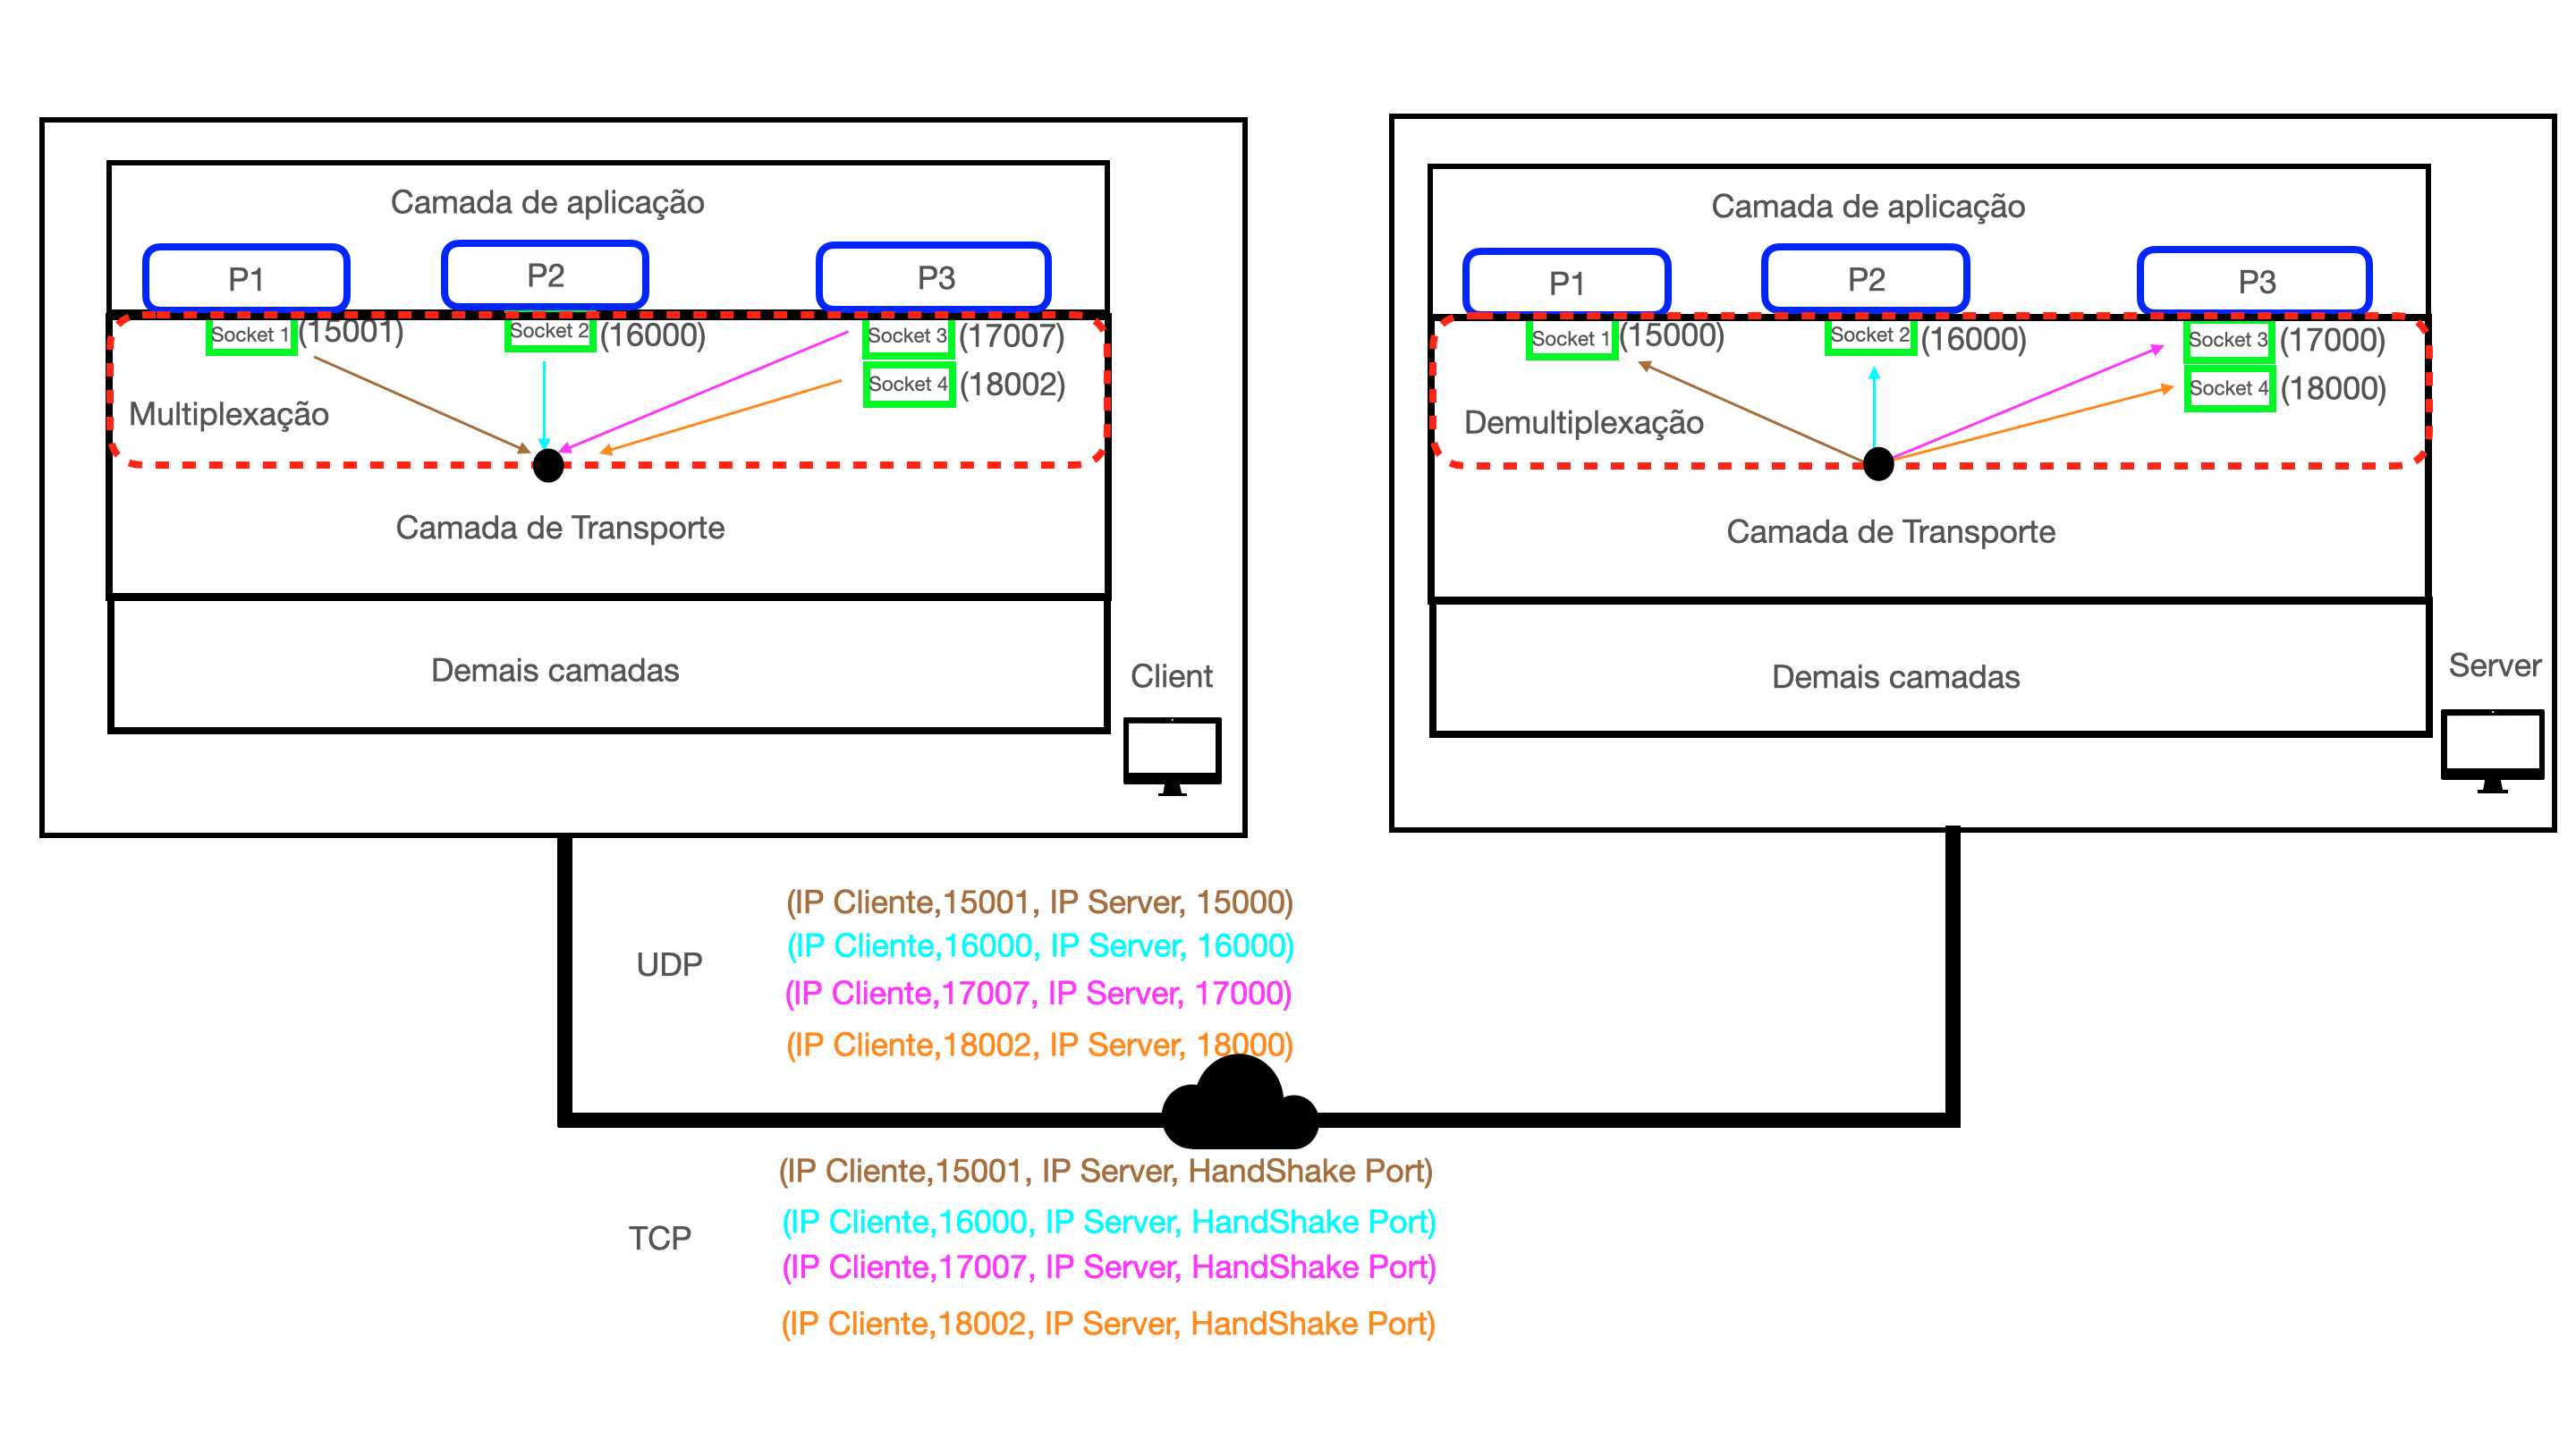
\includegraphics[keepaspectratio, width=16cm, height=12cm]{imagens/11/11 - Multiplexacao e Demultiplexacao.png}
\caption{Multiplexação e Demultiplexação\\}
\label{Multiplexação e Demultiplexação}
\end{figure}



Diferentemente do UDP, no qual a demultiplexação ocorre com o
encaminhamento dos dados diretamente para a porta de destino, descrita
no \emph{header} do \emph{segment}, (ou seja, o \emph{socket} UDP é
completamente identificável com \emph{2-tuple}, ou estrutura de dados
que contém o IP e \emph{port} de destino), o TCP necessita da
\emph{4-tuple} completa para a identificação do respectivo socket. Essa
abordagem simplifica a arquitetura \emph{client-server}, pois o servidor
pode utilizar de um única porta (como uma \emph{well-known port number},
número de porta que varia de 0 até 1023) para a execução do
\emph{handshaking}, como a 80 no caso do HTTP, enquanto que entrega
dinamismo à criação (ocorrendo no \emph{request}) e finalização dos
\emph{sockets}, algo que sucede o encerramento do canal de comunicação.
Na Figura \ref{Multiplexação e Demultiplexação} pode ser observado como os dados contidos na \emph{4-tuple}
podem variar conforme o protocolo escolhido.

É importante perceber que um processo pode ler e escrever no
\texttt{file\ descriptor} (\emph{socket}) criado para cada conexão
iniciada. E múltiplas conexões podem ser manipuladas por um único
processo, vinculando-se o \emph{socket} correspondente a uma thread
responsável pelo processamento das requisições do cliente. Desse modo,
um processo pode possuir múltiplos \emph{sockets} e interagir
individualmente com eles pelo \texttt{file\ descriptor} correspondente
na thread específica para a conexão em questão.

Dessa maneira, pode-se salientar uma forma de operação dos servidores,
no qual cada \emph{request} recebido gera um novo conjunto \emph{thread}
e \emph{socket} e o fim da conexão encerra esse conjunto. Portanto, o
período de vida do \emph{thread} e \emph{socket} pode ser longo, durando
toda a comunicação no modo persistente, ou curto, com a conexão
encerrando-se logo após o envio do \emph{response} no modo não
persistente. Requisições frequentes no modo não persistente podem
impactar no desempenho do sistema.

Como criar uma thread ou processo para cada requisição é
computacionalmente custoso, os \emph{servers} atuais implementam um
sistema produtor-consumidor, como mostrado na Figura \ref{Pool of Threads}, composto por
uma \emph{thread} produtora e um \emph{pool of threads} consumidoras. A
\emph{thread} produtora, vinculada à um \emph{socket}, recebe as
requisições oriundas dos \emph{clients} e deposita-os em uma fila
chamada \emph{task queue} (\emph{buffer}). Essas requisições serão
direcionadas para \emph{threads} consumidoras disponíveis, oriundas do
\emph{pool of threads}, as quais manterão-se ocupadas processando as
respectivas requisições coletadas (ou seja, não estarão disponíveis e,
portanto, não poderão adquirir novas requisições).

{[}Para saber mais, acesse:
https://httpd.apache.org/docs/2.4/mod/worker.html e
https://www.nginx.com/blog/thread-pools-boost-performance-9x/{]}


\begin{figure}[h!]
\centering
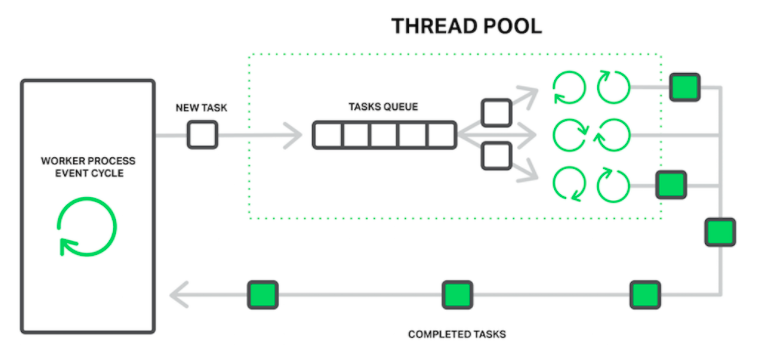
\includegraphics[keepaspectratio, width=12cm, height=9cm]{imagens/11/11 - pool of threads.png}
\caption{Pool of Threads \\
Imagem retirada de:
https://www.nginx.com/blog/thread-pools-boost-performance-9x/ em
05/12/2021. \\}
\label{Pool of Threads}
\end{figure}


\hypertarget{reliable-data-transfer-protocol}{%
\section {Reliable Data Transfer Protocol} \label{reliable-data-transfer-protocol}}

Para entender melhor sobre como funciona uma transferência de dados
confiável (\emph{Reliable Data Transfer Protocol}, RDT), será adotada
uma máquina computacional abstrada com um número finito de estados, no
qual assume somente um único estado por vez, chamada de Máquina de
Estados Finitos (\emph{Finite-State Machine}, FSM).

A cada nível de RDT será adicionado uma nova camada de complexidade, até
chegar no modelo mais próximo do real.

\hypertarget{rdt-1.0}{%
\subsection{RDT 1.0}\label{rdt-1.0}}

No primeiro caso, consideramos que as camadas mais baixas são
confiáveis. Ou seja não há perda ou alteração de dados e nem alteração
na ordem de envio. Assim:

Emissor:

\begin{enumerate}
\def\labelenumi{\arabic{enumi}.}

\item
  rdt\_send(data)
\item
  packet=make\_pkt(data)
\item
  udt\_send(packet)
\end{enumerate}

Receptor:

\begin{enumerate}
\def\labelenumi{\arabic{enumi}.}
\setcounter{enumi}{3}

\item
  rdt\_rcv(packet)
\item
  extract(packet,data)
\item
  deliver\_data(data)
\end{enumerate}

\hypertarget{rdt-2.0}{%
\subsection{RDT 2.0}\label{rdt-2.0}}

Em RDT 2.0, vamos considerar que, durante a transmissão, algum bit pode
ter sido corrompido. Assim, é necessário utilizar o protocolo ARQ
(\emph{Automatic Repeat reQuest}), o qual é baseado em três pontos:
detecção de erro, permitindo o receptor reconhecer a ocorrência de erro;
o \emph{feedback} do receptor, com o parecer positivo (equivalente à
``entendi!'') chamado de ACK ou negativo (equivalente à ``pode
repetir?''), denominado de NAK (em princípio, esse retorno basta ser de
1 bit de tamanho, sendo 0 para negativo e 1 para positivo); e
retrasmissão, com o emissor reenviando os pacotes caso tenha recebido
uma negativa (NAK) do receptor.

Emissor:

Envia os dados

\begin{enumerate}
\def\labelenumi{\arabic{enumi}.}
\tightlist
\item
  rdt\_send(data)
\item
  sndpkt = make\_pkt(data,checksum)
\item
  udt\_send(sndpkt)
\end{enumerate}

Espera por uma resposta\\
(reemissão em caso de NAK) 7. rdt\_rcv(rcvpkt) \&\& isNAK(rcvpkt)  \\
8. udt\_send(sndpkt)

(Encerra estado em caso de ACK)\\
9. rdt\_rcv(rcvpkt) \&\& isACK(rcvpkt)

Receptor: (Caso dados corrompidos)

\begin{enumerate}
\def\labelenumi{\arabic{enumi}.}
\setcounter{enumi}{3}
\tightlist
\item
  rdt\_rcv(rcvpkt) \&\& corrupt(rcvpkt)
\end{enumerate}

(Resposta)\\
5. sndpkt=make\_pkt(NAK) \\
6. udt\_send(sndpkt)

(Caso dados não-corrompidos)

\begin{enumerate}
\def\labelenumi{\arabic{enumi}.}
\setcounter{enumi}{3}
\tightlist
\item
  rdt\_rcv(rcvpkt) \&\& notcorrupt(rcvpkt)
\item
  extract(rcvpkt,data)
\item
  deliver\_data(data)
\end{enumerate}

(Resposta)\\
7. sndpkt = make\_pkt(ACK) 

8. udt\_send(sndpkt)

É importante perceber alguns detalhes desse protocolo. Primeiro, esse
protocolo é conhecido por \emph{stop-and-wait} pois o emissor não pode
receber nenhum comando do seu operador enquanto estiver esperando uma
resposta do receptor (novos comandos só correm quando a máquina estiver
em um estado apropriado). Segundo, não foi considerada a possibilidade
do ACK e NAK estarem corrompidos.

Para o segundo caso, há duas variações do RDT 2.0 no qual é implementado
um protocolo análogo ao incremento feito de RDT 1.0 para 2.0, chamados
de RDT 2.1 e 2.2.

\hypertarget{rdt-3.0}{%
\subsection{RDT 3.0}\label{rdt-3.0}}

Por fim, vamos considerar que poderá haver pacotes, ou suas respostas
ACK, perdidos durante a transmissão. A solução é o emissor esperar tempo
suficiente no qual garanta que os dados enviados ou respondidos foram
perdidos. Assim, caso o tempo seja ultrapassado, o emissor deve reenviar
os pacotes.

Como pode-se observar, não há como determinar um tempo ``garantidor'',
pois um atraso particularmente alto experimentado pelos pacotes pode ser
suficiente para ultrapassar o tempo estimado.

A determinação do tempo sofre de uma dicotomia, pois há vantagens e
desvantagens tanto com o aumento como com a diminuição do mesmo. Quanto
menor for o tempo, maior a chance de ocorrer falsas perdas (ocasionando
duplicações na emissão) por consequência de atrasos na rede. Porém,
incrementos nesse tempo podem impactar na velocidade da resposta do
emissor, pois o mesmo poderá ficar longos períodos de inatividade
aguardando uma resposta (perdida durante a transmissão). Assim, a
melhora na efetividade do protocolo passa pela determinação de um tempo
de espera ótimo (provavelmente desenvolvido para o atraso mais
frequente).

A Figura \ref{Protocolo RDT 3.0} mostra um exemplo do funcionamento do protocolo RDT 3.0
(também conhecido por \emph{alternating-bit protocol}, por causa da
alternância no número da sequência dos pacotes).

\begin{figure}[h!]
\centering
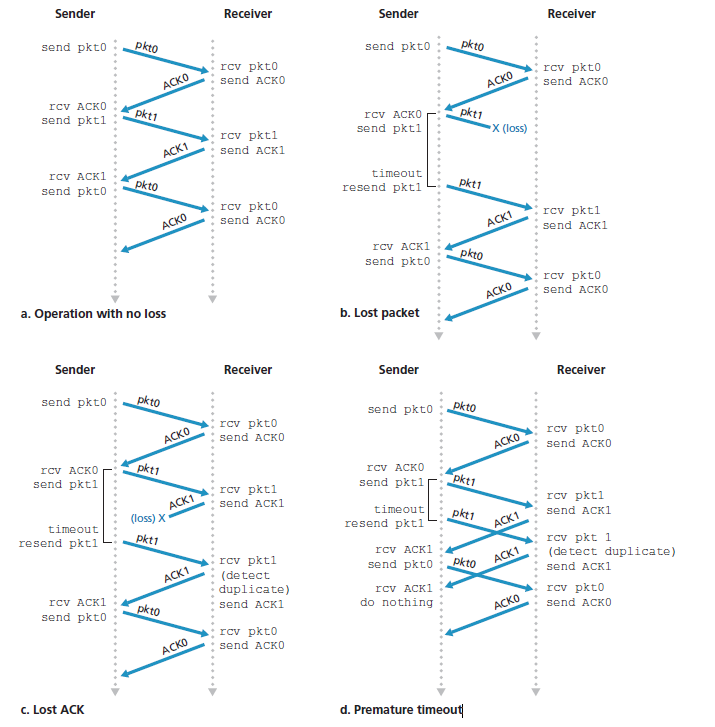
\includegraphics[keepaspectratio, width=14cm, height=17cm]{imagens/11/11 - rdt 3.0.png}
\caption{Protocolo RDT 3.0  \\
Imagem retirada de: Computer Networking a top-down approach. 8th
ed.~Pearson, página 212. \\}
\label{Protocolo RDT 3.0}
\end{figure}



\hypertarget{performance}{%
\subsection{Performance}\label{performace}}

O fundamento dos protocolos mencionados é enviar 1 pacote e esperar por
sua resposta. Uma forma de melhorar a performance é utilizar um padrão de
enviar múltiplos pacotes antes de entrar no estado de espera da resposta
de cada um, método chamado de \emph{pipeline}, como mostrado na Figura
\ref{Stop-and-wait vs pipelined}.


\begin{figure}[h!]
\centering
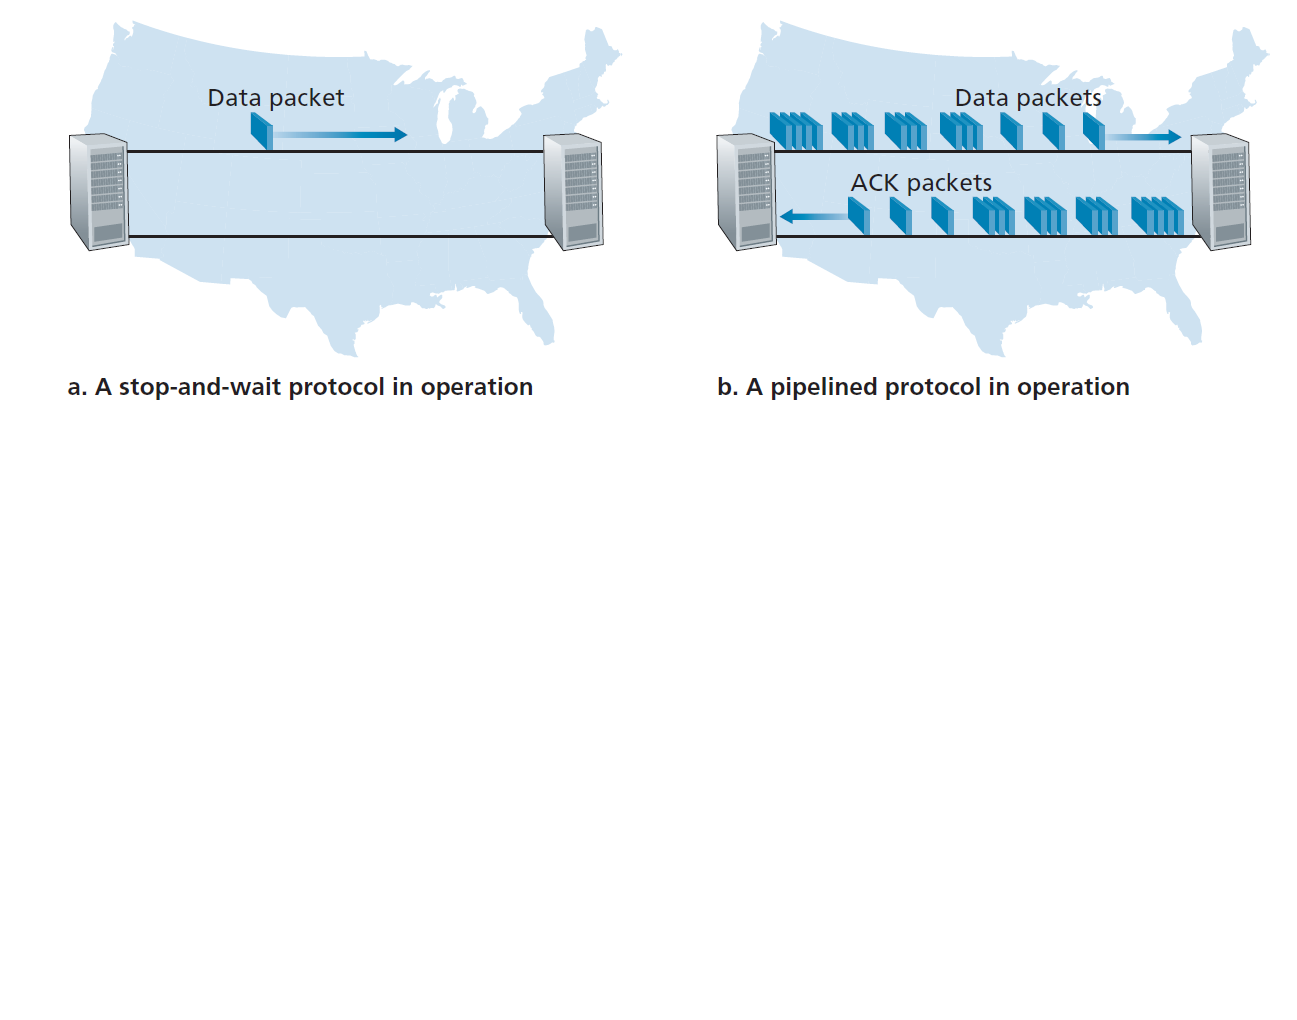
\includegraphics[keepaspectratio, width=14cm, height=11cm]{imagens/11/11 - stop and wait vs pipelined.png}
\caption{Stop-and-wait vs pipelined  \\
Imagem retirada de: Computer Networking a top-down approach. 8th
ed.~Pearson, página 213. \\}
\label{Stop-and-wait vs pipelined}
\end{figure}

Erros na abordagem do \emph{pipeline} são abordados nos protocolos
\emph{go-back-n} e \emph{selective repeat}, ambos tratados na próxima
aula.